\setcounter{section}{0}
\section{Trắc nghiệm}
\begin{enumerate}[label=\bfseries Câu \arabic*:]
	\item \mkstar{1}
	
	
	{Trong các chuyển động sau, chuyển động nào là đều?
		\begin{mcq}
			\item Chuyển động của quả dừa rơi từ trên cây xuống. 
			\item Chuyển đông của Mặt Trăng quanh Trái Đất. 
			\item Chuyển động của đầu cánh quạt.
			\item Chuyển động thực của chiếc xe buýt ở trên đường. 
		\end{mcq}
	}
	
	\hideall
	{		\textbf{Đáp án: B.}
		
		Chuyển đông của Mặt Trăng quanh Trái Đất là chuyển động đều.
		
	}
		\item \mkstar{2}
	
	
	{Trong các chuyển động sau, chuyển động nào được coi là rơi tự do? Tại sao?
		
		\begin{mcq}
			\item Chiếc lá đang rơi. 
			\item Hạt bụi chuyển động trong không khí. 
			\item Quả tạ rơi trong không khí. 
			\item Vận động viên đang nhảy dù. 
		\end{mcq}
		
	}
	
	\hideall
	{\textbf{Đáp án: C.}
		
		Trong câu A, lực cản không khí và trọng lượng chiếc lá gần như nhau nên chiếc lá đang rơi không được coi là rơi tự do.
		
		Trong câu B, ta thấy lực cản không khí lớn hơn rất nhiều so với trọng lượng của hạt bụi, nên hạt bụi chuyển động trong không khí không được coi là rơi tự do.
		
		Trong câu D, vận động viên đang nhảy dù có trọng lượng gần bằng lực cản không khí nên vận động viên đang nhảy dù không được coi là sự rơi tự do.
		
		Trong câu C, quả tạ có trọng lượng lớn hơn rất nhiều so với lực cản không khí nên quả tạ rơi trong không khí được coi là sự rơi tự do.
	
	}
	\item \mkstar{2}
	
	
	{Tàu Thống Nhất TN1 đi từ ga Huế vào ga Sài Gòn mất $\SI{20}{h}$. Biết vận tốc trung bình của tàu là $\SI{15}{m/s}$. Hỏi chiều dài của đường ray từ Huế vào Sài Gòn?
		\begin{mcq}(4)
			\item $\SI{3000}{km}$. 
			\item $\SI{1080}{km}$.
			\item $\SI{1000}{km}$.
			\item $\SI{1333}{km}$.
		\end{mcq}
	}
	
	\hideall
	{		\textbf{Đáp án: B.}
		
	Chiều dài của đường ray từ Huế vào Sài Gòn:
	$$s=vt=\SI{1080}{km}$$
		
	}
	\item \mkstar{2}
	
	
	{Trong trận đấu giữa Đức và Áo ở EURO 2008, tiền vệ Mai-cơn BaLack của đội tuyển Đức sút phạt cách khung thành của đội Áo $\SI{30}{m}$. Các chuyên gia tính được vận tốc trung bình của quả phạt đó lên tới $\SI{108}{km/h}$. Hỏi thời gian bay của quả bóng là bao nhiêu?
		\begin{mcq}(4)
			\item $\SI{1}{s}$. 
			\item $\SI{36}{s}$. 
			\item $\SI{1.5}{s}$.  
			\item $\SI{3.6}{s}$. 
		\end{mcq}
	}
	
	\hideall
	{\textbf{Đáp án: A.}
		
		Thời gian bay của quả bóng:
		$$t=\dfrac{s}{v} = 1\ \text s$$
		
	}
	\item \mkstar{2}
	
	
	{Hưng đạp xe lên dốc dài $\SI{100}{m}$ với vận tốc 2 m/s, sau đó xuống dốc dài $\SI{140}{m}$ hết 30 s. Hỏi vận tốc trung bình của Hưng trên cả hai đoạn đường?
		\begin{mcq}(4)
			\item $\SI{50}{m/s}$. 
			\item $\SI{8}{m/s}$. 
			\item $\SI{4.67}{m/s}$. 
			\item $\SI{3}{m/s}$.
		\end{mcq}
	}
	
	\hideall
	{\textbf{Đáp án: D.}
		
		Thời gian trên đoạn đường thứ nhất:
		$$t_1=\dfrac{s_1}{v_1} = 50\ \text s$$
		
		Vận tốc trung bình trên cả hai đoạn đường:
		$$v=\dfrac{s_1+s_2}{t_1+t_2} = 3\ \text {m/s}$$
		
	}
	\item \mkstar{2}
	
	
	{
		Một học sinh vô địch trong giải điền kinh ở nội dung chạy cự li $\SI{1000}{m}$ với thời gian là 2 phút 5 giây. Vận tốc của học sinh đó là
		\begin{mcq}(4)
			\item $\SI{40}{m/s}$. 
			\item $\SI{8}{m/s}$. 
			\item $\SI{4.88}{m/s}$. 
			\item $\SI{120}{m/s}$.
		\end{mcq}
	}
	
	\hideall
	{\textbf{Đáp án: B.}
		
		Vận tốc của học sinh đó là
		$$v=\dfrac{s}{t} = \SI{8}{m/s}$$
		
	}
	

	\item \mkstar{2}

	
	{Một người thả rơi một hòn bi từ trên cao xuống đất và đo được thời gian rơi là $\SI{3,1}{s}$. Bỏ qua sức cản không khí. Lấy $g = \SI{9,8}{m/s}^2$. Tính độ cao của nơi thả hòn bi so với mặt đất.
	\begin{mcq}(4)
		\item $\SI{47,089}{m}$. 
		\item $\SI{48,089}{m}$. 
		\item $\SI{49,089}{m}$. 
		\item $\SI{74,089}{m}$. 
	\end{mcq}
	
	}

	\hideall
	{\textbf{Đáp án: A.}
	
	Độ cao của nơi thả hòn bi so với mặt đất là:
	
	$$ h = \dfrac{1}{2}gt^2 = \SI{47,089}{m}.$$
	
	}
	
	\item \mkstar{2}
	
	
	{Một người thả rơi một hòn bi từ trên cao xuống đất và đo được thời gian rơi là $\SI{3,1}{s}$. Bỏ qua sức cản không khí. Lấy $g = \SI{9,8}{m/s}^2$. Tính quãng đường rơi được trong $\SI{0,5}{s}$ cuối trước khi chạm đất.
		\begin{mcq}(4)
			\item $\SI{47,089}{m}$. 
			\item $\SI{33,124}{m}$. 
			\item $\SI{33,089}{m}$. 
			\item $\SI{13,965}{m}$. 
		\end{mcq}
		
	}
	
	\hideall
	{\textbf{Đáp án: D.}
		
		Độ cao của nơi thả hòn bi so với mặt đất là:
		
		$$ h = \dfrac{1}{2}gt^2 = \SI{47,089}{m}.$$
		
		
		Thời gian bắt đầu rơi đến trước $\SI{0,5}{s}$ cuối trước khi chạm đất
		
		$$ t = \text{3,1} - \text{0,5} = \SI{2,6}{s}.$$ 
		
		Quãng đường vật rơi trong $\SI{2,6}{s}$ đầu là:
		
		$$h_1 = \dfrac{1}{2} gt^2 = \SI{33,124}{m}.$$
		
		Quãng đường vật rơi được trong $\SI{0,5}{s}$ cuối là: 
		
		$$h_2 = h - h_1 = \SI{13,965}{m}.$$
	
	}
	\item \mkstar{2}
	
	
	{Một người chạy xe máy theo một đường thẳng và có vận tốc theo thời gian được biểu diễn bởi đồ thị  ($v - t$) như hình. Xác định gia tốc của người này tại thời điểm 1 giây.
		
		\begin{center}
			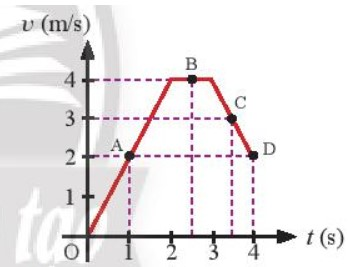
\includegraphics[scale=0.6]{../figs/VN10-2022-PH-TP0001-7.jpg}
		\end{center}

		\begin{mcq}(4)
			\item $\SI{2}{m/s}^2$. 
			\item $\SI{1,75}{m/s}^2$. 
			\item $\SI{1,6}{m/s}^2$.
			\item $\SI{2,75}{m/s}^2$.
		\end{mcq}
		
	}
	
	\hideall
	{\textbf{Đáp án: A.}
		
		Gia tốc của người này tại thời điểm 1 giây
		
		$$a = \dfrac{v_2 - v_1}{t_2 - t_1} = \SI{2}{m/s}^2.$$
		
	}
		\item \mkstar{2}
	
	
	{Một đoàn tàu đang chạy với vận tốc $\SI{43,2}{km/h}$ thì hãm phanh, chuyển động thẳng chậm dần đều để vào ga. Sau 1 phút thì tàu dừng lại ở sân ga. Tính quãng đường mà tàu đi được trong thời gian hãm phanh.
	
	
		\begin{mcq}(4)
			\item $\SI{380}{m}$. 
			\item $\SI{360}{m}$. 
			\item $\SI{120}{m}$. 
			\item $\SI{720}{m}$. 
		\end{mcq}
		
	}
	
	\hideall
	{\textbf{Đáp án: B.}
		
		Ta có: $v_0 = \SI{43,2}{km/h} = \SI{12}{m/s}$; $v = \SI{0}{m/s}$; $t = 1\ \text{phút} = \SI{60}{s}$.
		
		Gia tốc của tàu là:
		
		$$a = \dfrac{v - v_0}{t} = -\SI{0,2}{m/s}^2.$$
		
		Quãng đường mà tàu đi được là:
		
		$$d = \dfrac{v^2 - v_0^2}{2a} = \SI{360}{m}.$$
		
	}
	
	\item \mkstar{2}
	
	
	{Một máy bay chở khách đạt tốc độ cất cánh là $\SI{297}{km/h}$ ở cuối đoạn đường băng sau 30 giây từ lúc bắt đầu lăn bánh. Giả sử máy bay chuyển động thẳng, hãy tính gia tốc trung bình của máy bay trong quá trình này.
		

		\begin{mcq}(4)
			\item $\SI{1,75}{m/s}^2$.  
			\item $\SI{2,75}{m/s}^2$. 
			\item $\SI{3,75}{m/s}^2$.  
			\item $\SI{4,75}{m/s}^2$.  
		\end{mcq}
		
	}
	
	\hideall
	{\textbf{Đáp án: B.}
		
		Đổi $\SI{297}{km/h} = \SI{82,5}{m/s}.$
		
		Gia tốc trung bình của máy bay trong quá trình bay là:
		
		$$a = \dfrac{v_2-v_1}{t_2 - t_1} = \SI{2,75}{m/s}^2.$$
		
		
	}
	\item \mkstar{2}
	
	
	{Đồ thị ($v - t$) được biểu diễn trong hình. Đoạn nào thể hiện chuyển động nhanh dần đều?
		\begin{center}
			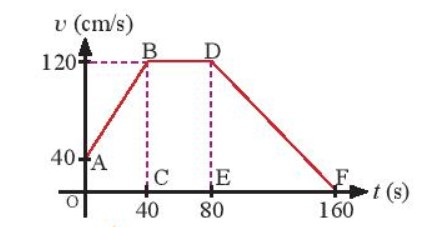
\includegraphics[scale=0.6]{../figs/VN10-2022-PH-TP0001-6.jpg}
		\end{center}	
		\begin{mcq}(4)
			\item AF. 
			\item DF. 
			\item BD. 
			\item AB. 
		\end{mcq}
		
	}
	
	\hideall
	{\textbf{Đáp án: D.}
		
		Độ dốc đi lên, vận tốc tăng dần theo thời gian, vật chuyển động nhanh dần đều. Nên từ A đến B, vật chuyển động nhanh dần đều.
		
		
	
		
	}
		\item \mkstar{2}
	
	
	{Đồ thị ($v - t$) được biểu diễn trong hình. Đoạn nào thể hiện chuyển động thẳng đều?
		\begin{center}
			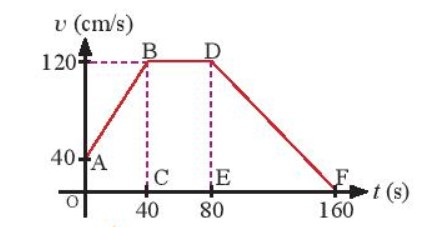
\includegraphics[scale=0.6]{../figs/VN10-2022-PH-TP0001-6.jpg}
		\end{center}	
		\begin{mcq}(4)
			\item AF. 
			\item DF. 
			\item BD. 
			\item AB. 
		\end{mcq}
		
	}
	
	\hideall
	{\textbf{Đáp án: C.}
		
		Từ B đến D, vật chuyển động thẳng đều. Do độ dốc nằm ngang, vận tốc không thay đổi theo thời gian, vật chuyển động thẳng đều.
		
	}
	
	\item \mkstar{2}
	
	
	{Trong giải đua F1, các tay đua phải hoàn thành một chặng đua dài khoảng $\SI{300}{km}$ trong khoảng thời gian ngắn nhất. Trong quá trình đua, các tay đua bắt buộc phải vào trạm dừng thay lốp mới và nạp thêm nhiên liệu. Trong khảng thời gian từ khi xe vào trạm dừng đến khi xe tăng tốc trở lại đường đua, ta thấy vận tốc của xe đã có sự thay đổi rõ rệt. Đại lượng nào đặc trưng cho sự thay đổi vận tốc của xe?
	
		\begin{mcq}(2)
			\item Gia tốc. 
			\item Thời gian. 
			\item Khối lượng. 
			\item Quãng đường. 
		\end{mcq}
		
	}
	
	\hideall
	{\textbf{Đáp án: A.}
		
		Đại lượng đặc trưng cho sự thay đổi vận tốc của xe là gia tốc.
		
	}
	\item \mkstar{2}
	
	
	{Một chiếc máy bay đang bay từ Thành phố Hồ Chí Minh đến Thủ đô Hà Nội với tốc độ $\SI{525}{km/h}$. Trong hôm đó, gió thổi về hướng Nam với tốc độ $\SI{36}{km/h}$. Xem như máy bay chuyển động thẳng đều theo hướng Bắc và quãng đường bay từ Thành phố Hồ Chí Minh đến Thủ đô Hà Nội là $\SI{1160}{km}$. Hãy xác định thời gian bay của máy bay trên quãng đường đó.
	
		\begin{mcq}(4)
			\item $\SI{3,27}{h}$. 
			\item $\SI{7,32}{h}$. 
			\item $\SI{1,37}{h}$. 
			\item $\SI{2,37}{h}$. 
		\end{mcq}
		
	}
	
	\hideall
	{\textbf{Đáp án: D.}
		
		Gọi:
		
		$\vec v_{1,2}$ là vận tốc của máy bay so với gió.
		
		
		$\vec v_{2,3}$ là vận tốc của gió so với mặt đất.
		
		
		$\vec v_{1,3}$ là vận tốc của máy bay so với mặt đất.
		
		Ta có:
		
		$$\vec v_{1,3} = \vec v_{1,2} + \vec v_{2,3}.$$
		
		Vận tốc của máy bay so với gió là $v_{1,2}= \SI{525}{km/h}$; vận tốc của gió so với mặt đất là $ v_{2,3}= \SI{36}{km/h}$.
		
		Chọn chiều dương là chiều chuyển động của máy bay (hướng bắc).
		
		Do gió chuyển động theo hướng nam nên: $\vec v_{2,3} <0$.
		
		Vận tốc của máy bay:
		
		$$v_{1,3} = v_{1,2} - v_{2,3} = \SI{489}{km/h}.$$
		
		Thời gian bay của máy bay trên quãng đường $\SI{1160}{km}$ là:
		
		$$ t =\dfrac{S}{v} \approx \SI{2,37}{h}.$$
	}
		\item \mkstar{2}
	
	
	{Một vật chuyển động thẳng có đồ thị ($d - t$) được mô tả như hình. Hãy xác định tốc độ tức thời của vật tại vị trí A.
		
		\begin{center}
			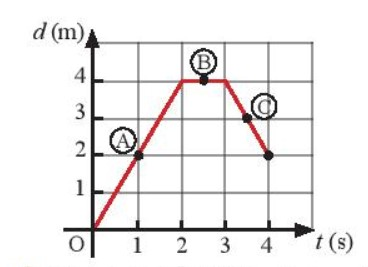
\includegraphics[scale=0.6]{../figs/VN10-2022-PH-TP0001-4.jpg}
		\end{center}	
		\begin{mcq}(4)
			\item $\SI{2}{m/s}$. 
			\item $\SI{1,6}{m/s}$. 
			\item $\SI{0,86}{m/s}$. 
			\item $\SI{32}{m/s}$. 
		\end{mcq}
	}
	
	\hideall
	{\textbf{Đáp án: A.}
		
		Tốc độ tức thời tại vị trí A:
		
		$$v_\text{A} = \dfrac{d_\text{A}}{t_\text{A}} = \SI{2}{m/s}.$$
		
	}
	\item \mkstar{2}
	
	
	{
		Một vật chuyển động thẳng có đồ thị ($d – t$) được mô tả như hình. Hãy xác định tốc độ tức thời của vật tại vị trí B.
		
		\begin{center}
		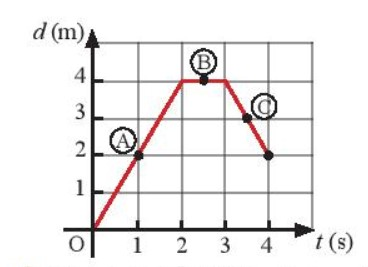
\includegraphics[scale=0.6]{../figs/VN10-2022-PH-TP0001-4.jpg}
		\end{center}	
		\begin{mcq}(4)
			\item $\SI{2}{m/s}$. 
			\item $\SI{1,6}{m/s}$. 
			\item $\SI{0,86}{m/s}$. 
			\item $\SI{32}{m/s}$. 
		\end{mcq}
		
	}
	
	\hideall
	{\textbf{Đáp án: B.}
		
		Tốc độ tức thời tại vị trí B:
		
		$$v_\text{B} = \dfrac{d_\text{B}}{t_\text{B}} = \SI{1,6}{m/s}.$$
		
	}
	\item \mkstar{4}

	
	{Một chiếc ô tô chạy từ điểm A đến điểm B. Nửa đoạn đường đầu ô tô đi với vận tốc $v_1=\SI{40}{km/h}$. Trong quãng thời gian còn lại thì một nửa quãng thời gian đầu ô tô đi với vận tốc $v_2=\SI{50}{km/h}$, một nửa quãng thời gian cuối ô tô đi với vận tốc $v_3=\SI{60}{km/h}$. Tính vận tốc trung bình của ô tô trên cả đoạn đường AB. 
	
	\begin{mcq}(4)
		\item $\SI{50.9}{km/h}$.	
		\item $\SI{55.7}{km/h}$.	
		\item $\SI{57.4}{km/h}$.	
		\item $\SI{58.5}{km/h}$.	
	\end{mcq}
	
	}

	\hideall
	{\textbf{Đáp án: C.}
	
	Vận tốc trung bình trên cả đoạn đường:
	$$v=\dfrac{2}{\dfrac{1}{v_1}+\dfrac{1}{v_2}}$$
	
	Vận tốc trung bình trên nửa đoạn đường thứ hai:
	$$v_2=\dfrac{v_2'+v_2''}{2} = \SI{55}{km/h}$$
	
	Vậy vận tốc trung bình trên cả đoạn đường:
	$$v=\SI{57.4}{km/h}$$
	}
	\item \mkstar{4}

	
	{Một chiếc ô tô chạy từ điểm A đến điểm B. Nửa quãng thời gian đầu ô tô đi với vận tốc $v_1=\SI{40}{km/h}$. Trong quãng thời gian còn lại thì một nửa quãng thời gian đầu ô tô đi với vận tốc $v_2=\SI{50}{km/h}$, một nửa quãng thời gian cuối ô tô đi với vận tốc $v_3=\SI{60}{km/h}$. Tính vận tốc trung bình của ô tô trên cả đoạn đường AB. 
	
	\begin{mcq}(4)
		\item $\SI{45.5}{km/h}$.	
		\item $\SI{47.5}{km/h}$.	
		\item $\SI{57.5}{km/h}$.	
		\item $\SI{55.5}{km/h}$.	
	\end{mcq}
	
	}
	
	\hideall
	{\textbf{Đáp án: B.}
	
	Vận tốc trung bình trên cả đoạn đường:
	$$v=\dfrac{v_1+v_2}{2}$$
	
	Vận tốc trung bình trên nửa quãng thời gian thứ hai:
	$$v_2=\dfrac{v_2'+v_2''}{2} = \SI{55}{km/h}$$
	
	Vậy vận tốc trung bình trên cả đoạn đường:
	$$v=\SI{47.5}{km/h}$$
	}
	\item \mkstar{4}

	
	{Một chiếc ô tô chạy từ điểm A đến điểm B. Nửa đoạn đường đầu ô tô đi với vận tốc $v_1=\SI{40}{km/h}$. Trong nửa đoạn đường còn lại thì một nửa đoạn đường đầu ô tô đi với vận tốc $v_2=\SI{50}{km/h}$, một nửa đoạn đường cuối ô tô đi với vận tốc $v_3=\SI{60}{km/h}$. Tính vận tốc trung bình của ô tô trên cả đoạn đường AB. 
	
	\begin{mcq}(4)
		\item $\SI{55.25}{km/h}$.	
		\item $\SI{50.15}{km/h}$.	
		\item $\SI{48.15}{km/h}$.	
		\item $\SI{46.15}{km/h}$.	
	\end{mcq}
	
	}

	\hideall
	{\textbf{Đáp án: D.}
	
	Vận tốc trung bình trên cả đoạn đường:
	$$v=\dfrac{2}{\dfrac{1}{v_1}+\dfrac{1}{v_2}}$$
	
	Vận tốc trung bình trên nửa đoạn đường thứ hai:
	$$v_2=\dfrac{2}{\dfrac{1}{v_2'}+\dfrac{1}{v_2''}} = \SI{54.54}{km/h}$$
	
	Vậy vận tốc trung bình trên cả đoạn đường:
	$$v=\SI{46.15}{km/h}$$
	}
	
	\end{enumerate}



\hideall
{
	\begin{center}
		\textbf{BẢNG ĐÁP ÁN}
	\end{center}
	\begin{center}
		\begin{tabular}{|m{2.8em}|m{2.8em}|m{2.8em}|m{2.8em}|m{2.8em}|m{2.8em}|m{2.8em}|m{2.8em}|m{2.8em}|m{2.8em}|}
			\hline
			1.B  & 2.C  & 3.B  & 4.A  & 5.D  & 6.B  & 7.A  & 8.D  & 9.A  & 10.B  \\
			\hline
			11.B  & 12.D  & 13.C  & 14.A  & 15.D  & 16.A  & 17.B  & 18.C  & 19.B  & 20.D  \\
			\hline
			
		\end{tabular}
	\end{center}
}
\section{Tự luận}
\begin{enumerate}[label=\bfseries Câu \arabic*:]
		\item \mkstar{2}
	
	{
		Bạn C đứng yên trên sân ga vẫy tay tiễn bạn A và bạn B trên tàu hỏa. Khi tàu chuyển động, bạn C thấy bạn B đang chuyển động ra xa trong khi bạn A lại thấy bạn B đứng yên trên tàu. Tại sao?
		\begin{center}
			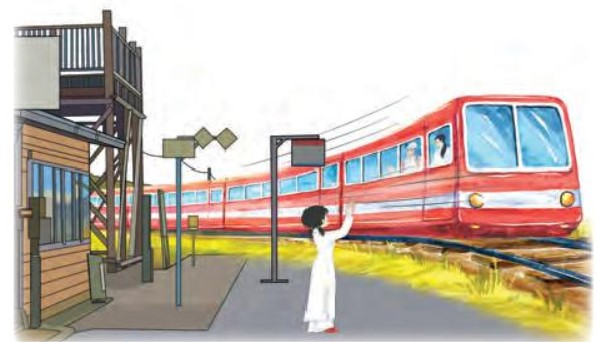
\includegraphics[scale=0.6]{../figs/VN10-2022-PH-TP0001-5.jpg}
		\end{center}	
		
	}
	
	\hideall{
		
	Bạn C thấy bạn B đang chuyển động trong khi đó bạn A lại thấy bạn B đứng yên, sở dĩ như vậy là do tính tương đối của chuyển động, tùy vào vật được họn làm mốc.
	

	}
	\item \mkstar{2}
	
	{
	Thả rơi tự do một vật khối lượng $\SI{2}{kg}$ từ độ cao $\SI{180}{m}$ xuống mặt đất, Lấy $g = \SI{10}{m/s}^2$.
		\begin{enumerate}
			\item Tính quãng đường vật rơi được trong giây cuối cùng.
			\item Tính vận tốc của vật trước khi vật chạm đất 2 giây.
		\end{enumerate}
	}
	
	\hideall{
	
	\begin{enumerate}
		\item 
		Thời gian bắt đầu rơi đến lúc chạm đất
		
		$$h = \dfrac{1}{2}gt^2 \Rightarrow t = \SI{6}{s}.$$
		
		Quãng đường vật rơi được trong giây cuối cùng
		
		$$s_6 = \dfrac{1}{2} g(6^2 - 5^2) = \SI{55}{m}.$$
		
		\item Vận tốc của vật trước khi vật chạm đất 2 giây
		
		$$v = gt = g(6-2) = \SI{40}{m/s}.$$
	\end{enumerate}
	}
	
	\item \mkstar{2}
	
	
	{Một người đi xe đạp thả dốc xuống một cái dốc dài $\SI{120}{m}$ hết $\SI{30}{s}$. Khi hết dốc, xe lăn tiếp trên quãng đường nằm ngang dài $\SI{60}{m}$ trong $\SI{24}{s}$ rồi dừng lại. Tính vận tốc trung bình của xe đạp trên quãng đường xuống dốc, trên đoạn đường nằm ngang và trên cả hai đoạn đường.
	}
	
	\hideall
	{Vận tốc trung bình trên quãng đường xuống dốc:
		$$v_1 = \dfrac{s_1}{t_1} = \SI{4}{m/s}$$
		
		Vận tốc trung bình trên quãng đường nằm ngang:
		$$v_2 = \dfrac{s_2}{t_2} = \SI{2.5}{m/s}$$
		
		Vận tốc trung bình trên cả hai đoạn đường:
		$$v= \dfrac{s_1 + s_2}{t_1 + t_2} = \SI{3.3}{m/s}$$
	}
		\item \mkstar{3}
	
	
	{
		Một máy bay đang bay ở độ cao 5 km với tốc độ $\SI{500}{km/h}$ theo phương ngang thì thả rơi một vật. Hỏi người lái bay phải thả vật cách mục tiêu bao xa theo phương ngang để vật rơi trúng mục tiêu? Lấy $g = \SI{9,8}{m/s}^2$ .
		
		
	}
	
	\hideall
	{
		Ta có:
		
		$$v_0 = \SI{500}{km/h} = \SI{138,89}{m/s}.$$
		
		$$h = \SI{5}{km} = \SI{5000}{m}.$$
		
		Người lái máy bay phải thả vật cách mục tiêu là:
		
		$$L = v_0 \sqrt{\dfrac{2h}{g}} \approx \SI{4436,68}{m}.$$
		
		
	}
		\item \mkstar{3}
	
	
	{
		Một người lái xe ô tô đi thẳng $\SI{6}{km}$ theo hướng Tây, sau đó rẽ trái đi thẳng theo hướng nam $\SI{4}{km}$ rồi quay sang hướng Đông đi $\SI{3}{km}$. Xác định quãng đường đi được và độ dịch chuyển của ô tô.
	}
	
	\hideall
	{
		Quãng đường đi được của ô tô là: 
		
		$$6 + 4 + 3 = \SI{13}{km}.$$
		

	\begin{center}
	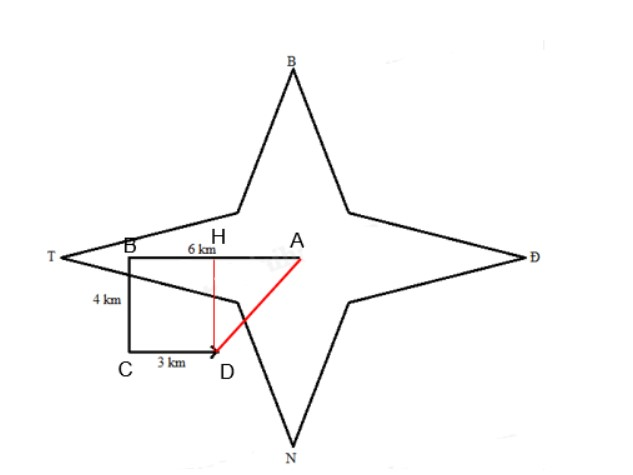
\includegraphics[scale=0.6]{../figs/VN10-2022-PH-TP0001-1.jpg}
	\end{center}	

		Độ dịch chuyển: AD
		
		Ta có: BH = CD = $\SI{3}{km}$; HD = BC = $\SI{4}{km}$; AH = AB - BH = 6 - 3 = $\SI{3}{km}$.
		
		$$\Rightarrow \text{AD} = \sqrt{\text{AH}^2 + \text{HD}^2} = \SI{5}{km}.$$
		
	
	}
	
	
\end{enumerate}